Die beiden Convolutional Direct Cascade Netzwerke unterscheiden sich ausschließlich darin, ob die Eingabedaten in ein- oder zweidimensionaler 
Form verarbeitet werden. Es lässt sich jedoch erkennen, dass die zweidimensionale Variante eine leicht bessere Performanz erzielt.

Der Grund dafür liegt in der Art der Filteroperationen: Während das eindimensionale Netzwerk in den Convolutional Layern lediglich benachbarte 
Datenpunkte entlang einer Achse berücksichtigt, kann das zweidimensionale Netzwerk zusätzlich auf Informationen aus vertikalen sowie diagonalen 
Nachbarschaften zugreifen. Dadurch wird eine umfassendere Erfassung lokaler Bildstrukturen ermöglicht.

Der Leistungsunterschied bleibt jedoch gering, wie in Abbildung \ref{fig:dim} dargestellt.

\begin{figure}[htpb]
    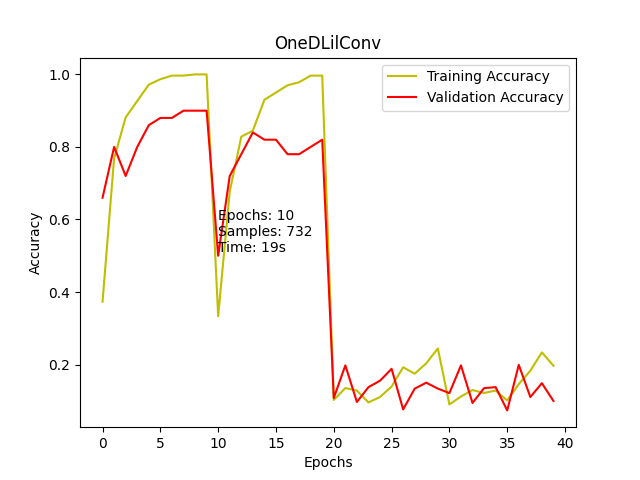
\includegraphics[height=5cm]{../../Plots/ba_plots/dimensionality/1dim_tr.png}
    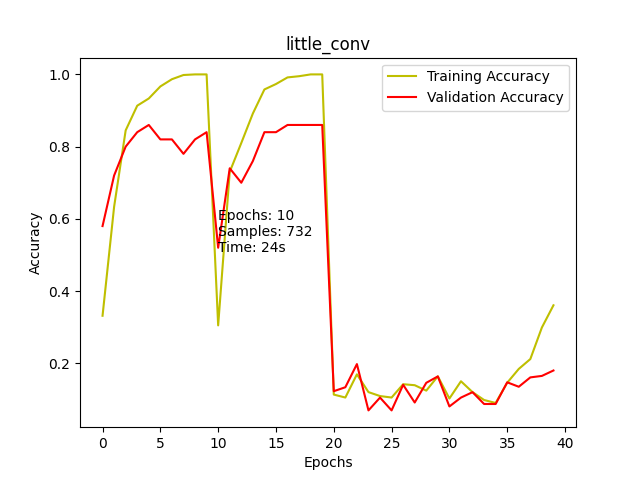
\includegraphics[height=5cm]{../../Plots/ba_plots/dimensionality/2dim_tr.png}
    \caption{\label{fig:dim} 
    \small{In der Abbildung sind links die Ergebnisse des Tests 1DC:TF2/732/10 und rechts jene von 2DC:TF2/732/10 dargestellt. Ziel dieser 
    Gegenüberstellung ist es, einen möglichst geringen Unterschied in der Performanz zwischen beiden Netzwerkarchitekturen nachzuweisen, um 
    die weitere Analyse auf das 1DC-Netzwerk beschränken zu können.}}
\end{figure}

Da das zweidimensionale Netzwerk aufgrund technischer Einschränkungen nur mit einer begrenzten Datenmenge eingesetzt werden kann, sollte es in 
diesem Fall eine deutlich kürzere Trainingszeit aufweisen. 
Die längere Dauer resultiert daraus, dass die Berechnung des Augmented Vectors einen erheblichen Zeitaufwand erfordert und gleichzeitig die 
Hauptursache für die Einschränkungen darstellt, da während der Berechnung Speicherplatzengpässe im Arbeitsspeicher auftreten.

Da der Unterschied in der Performanz zwischen ein- und zweidimensionalem Netzwerk lediglich marginal ist, genügt es in den meisten Fällen, das 
eindimensionale Netzwerk für die Analyse heranzuziehen. Die damit verbundenen technischen Limitationen des zweidimensionalen Netzwerks stellen 
somit kein wesentliches Hindernis für die Evaluation des TFs dar.
